\chapter{Experiments and results} \label{results}

\section{Experimental settings} 

In this particular experimental scenario, the basic guidelines 
proposed in Adomavicius \cite{adomavicius2011context} are followed,  
and they are briefly explained next. 
\begin{itemize} 
\item \textbf{Hypothesis:} before running the experiment we must form
an \textit{hypothesis}. It is important to be concise and restrictive
about this hypothesis, and design an experiment that tests the
hypothesis. For example, an hypothesis can be that  \textbf{algorithm
A} predicts better user ratings than  \textbf{algorithm B}.  In that
case, the experiment should test the prediction accuracy, and not
other factors.
\item \textbf{Controlling variables:} when comparing a few candidate
algorithms on a certain hypothesis, it is important that all
\textit{variables} that are not tested will stay fixed. For example,
suppose that we wish to compare the prediction accuracy of movie
ratings of  \textbf{algorithm A} and \textbf{algorithm B}, that both
use different collaborative filtering models.
\item \textbf{Generalization power:} when drawing conclusions from
experiments, we may desire that our conclusions generalize beyond the
immediate context of the experiments. When choosing an algorithm for a
real application, we may want our conclusions to hold on the deployed
system, and generalize beyond our experimental data set. Similarly,
when developing new algorithms, we want our conclusions to hold beyond
the scope of the specific application or data set that we experimented
with. It is important to understand the properties of the various data
sets that are used. Generally speaking, \textit{the more diverse the
data used, the more it can generalize the results}.
\end{itemize} 

\subsection{Off-line experiments} 

An off-line experiment is performed using a pre-collected dataset
of users choosing or ratings. Using this dataset tries to simulate
the behavior of users that interact with a recommender system. In
doing so, it assume that the user behavior when the data was collected
will be similar enough to the user behavior when the recommender
system is deployed, so that we can make reliable decisions based on
the simulation.  Off-line experiments are attractive because they
\textit{require no interaction with real users}, and thus it allows to compare
a wide range of candidate algorithms at a low cost. \\ The downside is
that it can answer a very narrow set of questions, typically questions
about the prediction of an algorithm. The goal of the off-line
experiments is to filter out inappropriate  approaches, leaving a
relatively small set of alternatives algorithms for subsequently to be
tested for the more costly user studies or on-line 
experiments\cite{adomavicius2011context}.\\ 
The next section shows a comprehensive description of the 
experimental setup for experiments, as well as results obtained 
in the experiments.
Each method was tested using contextual datasets in the domain. 
Results are showed in order to  compare the performance of the 
algorithms in the method. 
%% Haz un puente, dices que vaz a hacer ciertos experimentos
%% menciona aquí que lo que sigue es el setup de tus parte experimental.
%% Menciona brevemente los experimentos o datrasets, Restaurants, MovieLens,
%% Filmtrust and InCarMusic, TripAdvisor
<<<<<<< HEAD

%% Datasets?? esto ya está en la sección pasada
%% Ok, menciona que para poder hacer los experimentos los 
%% siguientes datasets fueron utilizados, pero justifica cada uno.

\section{Datasets} 

\subsection{Tijuana Restaurants} 
=======
%\section{Experiments} 
>>>>>>> origin/master
%% Esto creo que ya se había dicho,
%% o debe ir en Method
\section{Restaurant recommendations} 

The method uses collaborative filtering to find restaurants for the
user\cite{ramirez2013restaurant}. The ratings of user profiles are
used to determine the similarity among users using Pearson
correlation.\\ The similarity between the user and  neighbors is
used to calculate a weighted average of ratings for each particular
item;  the top-N ratings are used as a list of recommended restaurants
for the active user. The output of the collaborative filtering
algorithm (top-N list) is supplied to the next step of the 
post-filtering process. \\The restaurants are adjusted to the context in
the next step in order to make ranking of restaurants in the current
context. Post-filtering is based on the average of ratings in a
specific context, so prediction is made with: 1) the average post-
filtering a restaurant has in the current context (that is the mean of
user ratings) and 2) the rating predicted by the collaborative
filtering algorithm. The top-N list contains the restaurants with
highest predictions, so each restaurant is adjusted for the user’s
context and listed in contextual recommendations; the process is
depicted in figure \ref{fig:postfiltering}.

\begin{figure*}
\centering
\captionsetup{font=footnotesize}
\setlength\fboxsep{0pt}
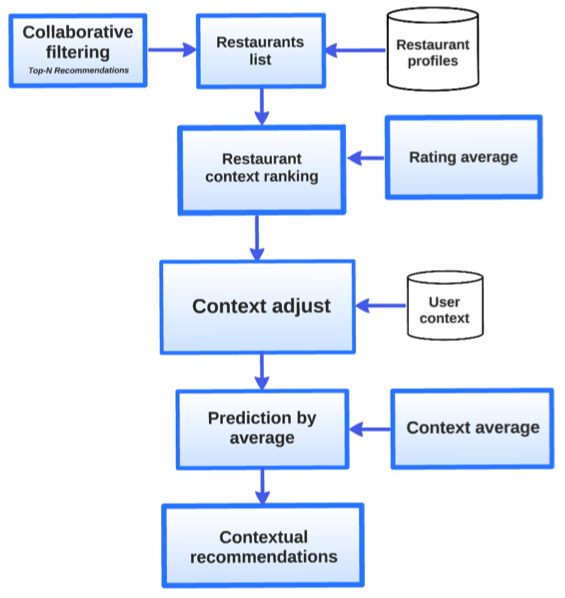
\includegraphics[width=0.50\textwidth]{img/posfil.png}
\caption{The post-filtering approach for Tijuana restaurants.}
\label{fig:postfiltering}     
\end{figure*}
%% Bien, empieza aquí:
%Algo como
<<<<<<< HEAD
%In order to validate  the proposed approach described in section XXX,
% Pero es muy general, ¿Qué es lo que vamos a validar?
% El desempñeo del algoritmo?
% La usabilidad del sistema?
% Comparar con contexto vs sin Contexto?
% Creo que es: Para validar el algoritmo de recomendación contextual
% en el dominio de los restaurantes
=======
%In order to validate the proposed approach described in section XXX, data about restaurant
>>>>>>> origin/master
In order to validate the proposed approach, data about restaurant
preferences of users in different contexts was collected. The study
subjects were students  with a major in engineering,  
master’s program and professors of the Tijuana Institute of
Technology. A total of \textit{50 users} answered a questionnaire; the
questions were about their preferences for nearby restaurants and the
technology most often used by them. The \textit{questionnaire} consisted 
of \textit{8 questions} and also they were asked to rate any number of restaurants from a list of 40 restaurants.
Each of the restaurants chosen, was rated 6 times one per proposed 
context, a matrix rating with \textit{1,422 ratings} was collected. The
questions are shown in table \ref{tab:questions}. The reason for allowing
<<<<<<< HEAD
users to chose what restaurants to rate was to give them the same liberty
they would when they visit a web or mobile application, in this case 
users are asked to rate only their favorite restaurants.

%Justificar el cuestionario
%Also a questionnaire was applied to participants in order to
=======
users to chose what restaurants to rate it to give them the same liberty
they have when visiting a web or mobile application. 
>>>>>>> origin/master
\begin{table}
\small
\captionsetup{font=footnotesize}
\caption{Questionnaire applied to participants.}
\label{tab:questions} 
\centering
\small
\begin{tabular}{p{7cm} p{5cm} }
\hline\noalign{\smallskip}
Question & Answers \\
\noalign{\smallskip}\hline\noalign{\smallskip}
\small{1.What is your occupation?} & \small{1. Student 2.Employee} \\ \hline  
\small{2.According to your priorities, order by importance the features 
you consider most when choosing a restaurant. } & 
\small{1.Installation/decoration 2.Prices 3.Service 4.Dishes 
5.Atmosphere 6.Location}  \\ \hline 
\small{3.What are the devices that you have?}
& \small{1.Smartphone 2.Tablet 3.Laptop 4.PC} \\ \hline   
\small{4.What Operating System do you use?} & 
\small{1.Android 2.Windows 3.iOS 4.Symbian 5.Blackberry 6.Other}
\\ \hline  
\small{5.If you do, What application to search restaurants in Tijuana do you use?} &
\small{1.Yes 2.No 3.Which one?} \\ \hline   
\small{6.Would you like to use an application of
recommender systems of Tijuana?} & \small{1.Yes 2.No} \\ \hline  
\small{7.Please, rate your favorites restaurants(without context).} & 
\small{Restaurant list} \\ \hline
\small{8.Please, rate your favorites restaurants in each contextual situation.} & 
\small{Restaurant list} \\
\noalign{\smallskip}\hline
\end{tabular}
\end{table}

The user's answers from question 1 to question 6 are represented in
the figure \ref{fig:cakeschart}. \textit{Figure \ref{fig:cakeschart}a}
represents the percentage of surveyed students and teachers;
\textit{figure \ref{fig:cakeschart}b}  the percentage of the element
that users consider the most important to visit a restaurant;
\textit{figure \ref{fig:cakeschart}c} represents the preferences of
devices when are using Internet for restaurant recommendations;
\textit{figure \ref{fig:cakeschart}d} represents the percentage of
operating system that often used, \textit{figure
\ref{fig:cakeschart}e} shows the percentage of users that use the
Internet to search restaurants in Tijuana; and \textit{figure
\ref{fig:cakeschart}f}, shows the percentage of users that would like
using a restaurant recommender system of Tijuana.
\begin{figure*}
\captionsetup{justification=centering,margin=2cm,font=footnotesize}
\centering
\setlength\fboxsep{0pt}
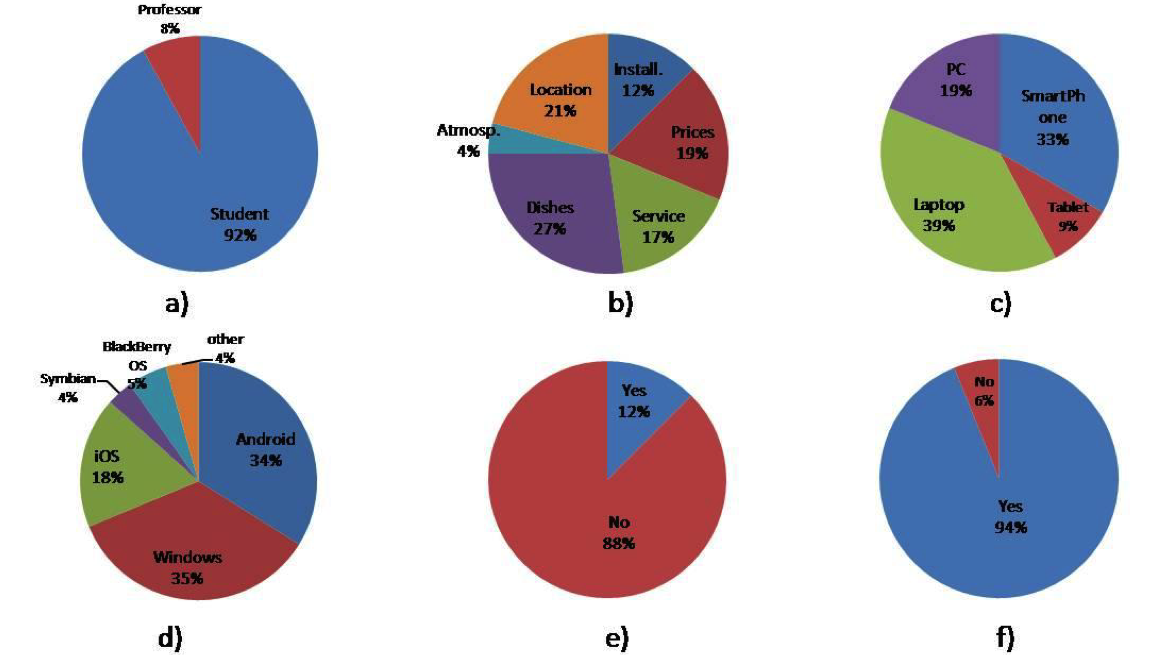
\includegraphics[width=0.8\textwidth]{img/cakes.png}
\caption{The chart shows user\'s preferences for questions 1 to 6.}
\label{fig:cakeschart}     
\end{figure*}
For questions 7 and 8 only the top-ten restaurants are shown,
without/with the contextual situation. In figure \ref{fig:barschart}a ,
the favorite restaurant is \textbf{Daruma}(178 votes),  whereas in
figure \ref{fig:barschart}b, \textbf{Daruma} does not appear in the
top-ten. When considering the context \textit{midweek}, the favorite
restaurant was \textbf{Carl's Jr.}, which appears in both graphs; this
restaurant was also the most voted in the different contexts.
\begin{figure*}
\captionsetup{justification=centering,margin=2cm,font=footnotesize}
\centering
\setlength\fboxsep{0pt}
%\setlength\fboxrule{0.7pt}
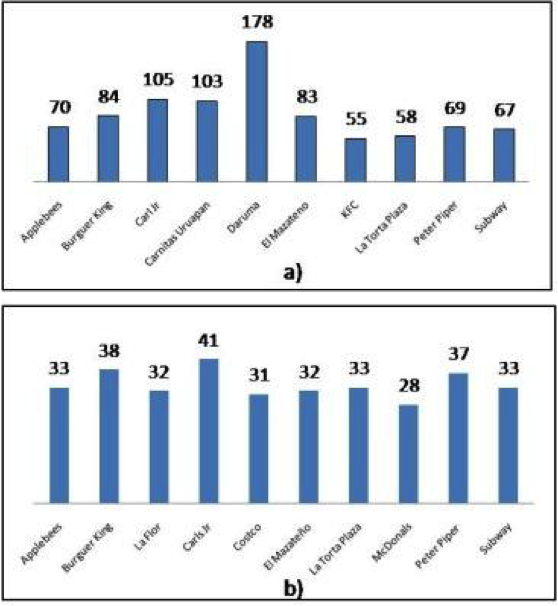
\includegraphics[width=0.55\textwidth]{img/bars.png}
\caption{The chart shows the users preferences for questions 7 and 8.}
\label{fig:barschart}     
\end{figure*}
Contextual recommendations of post-filtering approach depends of
context \textit{midweek} or \textit{weekend}, which is the day when
the restaurants were rated. Subsequently, the result of the query is
refined according to the user context; the 6 contexts mentioned
correspond to combinations of contextual factors shown in table
\ref{tab:contextstijuana}.
\begin{table}
\small
\captionsetup{font=footnotesize}
\caption{Contextual factors considered in the questionnaire.}
\label{tab:contextstijuana} 
\centering
\begin{tabular}{p{2.5cm} p{7cm} }
\hline\noalign{\smallskip}
Contextual Factor & Context \\
\noalign{\smallskip}\hline\noalign{\smallskip}
\small{Day} & \small{1.Midweek(Monday, Thuesday,Wednesday and Thursday)
2.Weekend(Friday,Saturday and Sunday)}  \\ \hline 
\small{Place} & \small{1.School 2. Home 3.Work} \\ 
\noalign{\smallskip}\hline
\end{tabular}
\end{table}

%%Que haces con este dataset?
%%Alguna conclusion?


% este es otro dataset?
% creo que es el mismo, corrige o borra el párrafo que sigue
% ya sabemos que fué explícito y fueron 50 usuarios
<<<<<<< HEAD
The dataset was explicitly collected from \textbf{50 users} who
answered the questionnaire (see table \ref{tab:questions}). A total of 172
predictions was made for different users and the mean absolute error
\textbf{MAE=0.5859} when the context \textbf{midweek} for the current user
was considered. The observation for this result is that using a small
dataset the performance of the method proposed is limited. On the other
hand, having only one contextual factor does not improve the accuracy
of the recommendations in this domain.
% Arriba ¿Por qué solo consideras esa predicción la de midweek?
=======
%The dataset was explicitly collected from \textbf{50 users} whom
%answered questionnaire (see table \ref{tab:questions}). 
A total of 172 predictions was made for different users and the 
mean absolute error \textbf{MAE=0.5859} when the context 
for the current user was considered. 
The observation for this result is that using a small
dataset the performance of the method proposed is limited. On the other
hand, having only one contextual factor does not improve the accuracy
of the recommendations in this domain.
%CHECAR EL ARTICULO
% Arriba ¿Por qué solo consideras esa prediccióm la de midweek?
>>>>>>> origin/master
% ¿ Por qué no otos casos o una tabla?
% ¿Cual es la hipotesis, variables etc.?
%%Explica que vas a hacer, no empieces por los datos, antes dí que vas a hacer
%%Que vas a utilizar y ya despué entras en el detalle de Movie Lens. 
\subsection{MovieLens collection} 
<<<<<<< HEAD
GroupLens Research has collected and made available rating data sets
from the MovieLens web site (\url{http://movielens.org}). \\The data sets
were collected over various periods of time,  depending on the size of
the set.
\begin{itemize} 
\item \textit{MovieLens 1M}: Stable benchmark dataset, 
1 million ratings from 6000 users on 4000 movies.
Released 2/2003.\\ Downloaded from
\url{http://grouplens.org/datasets/movielens/1m/}. 
\item \textit{MovieLens 10M}: Stable benchmark dataset, 
10 million ratings and 100,000
tag applications applied to 10,000 movies by 72,000 users. 
Released 1/2009. \\Downloaded from
\url{http://grouplens.org/datasets/movielens/10m/}. 
\end{itemize}

%%
%% Justifica antes que vas a probar, para que, después hablas del data set y los resultados.
=======
>>>>>>> origin/master

The proposed method for MovieLens uses post-filtering 
and time segmentation.
Time in recommender systems is used as a contextual factor in the
research reviewed \cite{baltrunas2009context},
\cite{baltrunas2009towards}, \cite{koren2010collaborative}, and
\cite{he2009time}, results vary according the techniques that were
done.\\  In \cite{he2009time} the pre-filtering approach was used, time
was divided in time intervals and the size of time intervals is
directly proportional to the distance from initiating the historical
information to the current user context. In
\cite{koren2010collaborative} a tracking model of user behavior over
the life-time of data is proposed, in order to exploit the relevant
components of all  data instances, while discarding only what is
modeled as being irrelevant.\\In \cite{baltrunas2009context} it is
shown that the time division is beneficial and its performance depends
on the items selection method and influence of contextual variables in
item ratings. In \cite{baltrunas2009towards} the user profile is
segmented into micro-profiles corresponding to a particular context,
each context represents a time span in which recommendations for users
are derived.\\This experiment implements fuzzy logic on time
segmentation, in order to improve user satisfaction by providing
recommendations based to context and recents user preferences without
discarding tastes in the past, as they include important information
for the recommender system proposed. \\The first phase is division of
three time segments based on the current context of the user is
performed such as in is depicted in figure \ref{fig:context-ml}.
\begin{figure*}
\captionsetup{justification=centering,margin=2cm,font=footnotesize}
\centering
\setlength\fboxsep{0pt}
%\setlength\fboxrule{0.7pt}
\fbox{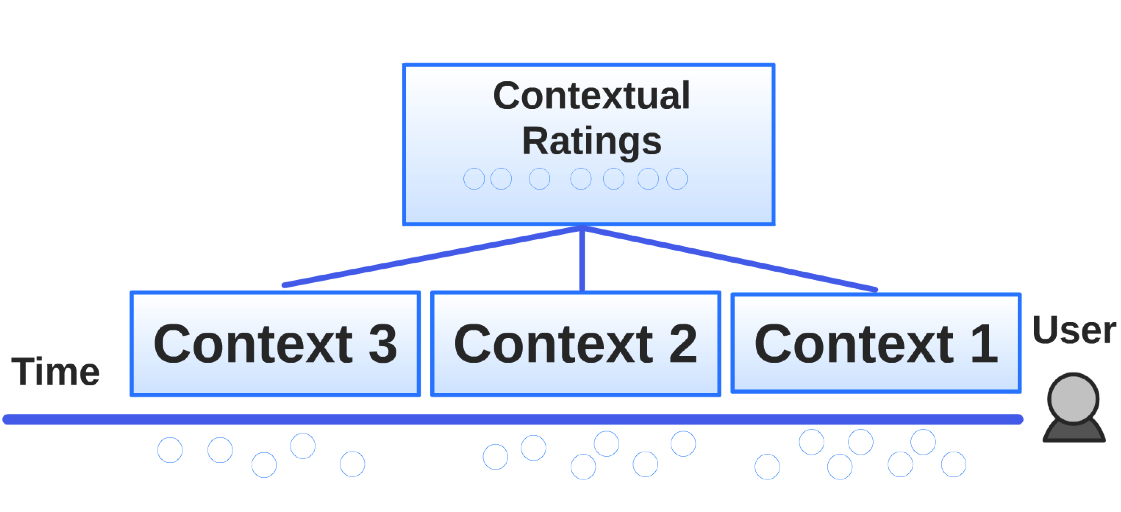
\includegraphics[width=0.50\textwidth]{img/context-ml.png}}
\caption{Time segmentation of contexts based on current user
context.}
\label{fig:context-ml}     
\end{figure*}
In recommender system, the first step is to obtain the user context, 
from this information three contexts
(figure \ref{fig:context-ml}) will be obtained that representing a
time segment of three months each one, in total the algorithm
considers all the ratings users did during nine months prior the
current context. Subsequently, ratings are classified by contexts and
reused as contextual rating matrix being, a ratings matrix for each
context. \\The size of matrix depends of users' participation during
the last nine months. One of the aims is to identify the user behavior
through recent information, in order to, for instance, know whether
the user changes ratings constantly; whether usually assign high, low
or mixed ratings; whether user likes to see different items or whether
have a favorite category.\\  Recommender systems use the collaborative
filtering algorithm in order to find relevant items for the user
\cite{ramirez2013restaurant}. User's profiles are used for determine
the similarity between users calculated with Pearson correlation. The
similarity between users can provide valuable information as long as
user participation is enough (less than 10 ratings). The next step is
to obtain recommendations list (Top-N), three contextual lists are the
outputs of collaborative filtering algorithm and contain items with
user's predictions for each context.\\Popularity's prediction
considers other variables: 1) user’s participation in respect of an
item in the context and, 2) the rating's average that users have given
for item in the same context. \\A Fuzzy Inference System (FIS) uses
these parameters to assign a weight within a scale from 1 to 5
(prediction value). These recommendations are used when the ratings
matrix is sparse, a popularity prediction is done. \\Finally, the
system gets the recommendations list for each user in different
contexts. The recommendation process for pre-filtering approach
 is depicted in figure \ref{fig:archi-ml}.
\begin{figure*}
\captionsetup{justification=centering,margin=2cm,font=footnotesize}
\centering
\setlength\fboxsep{0pt}
%\setlength\fboxrule{0.7pt}
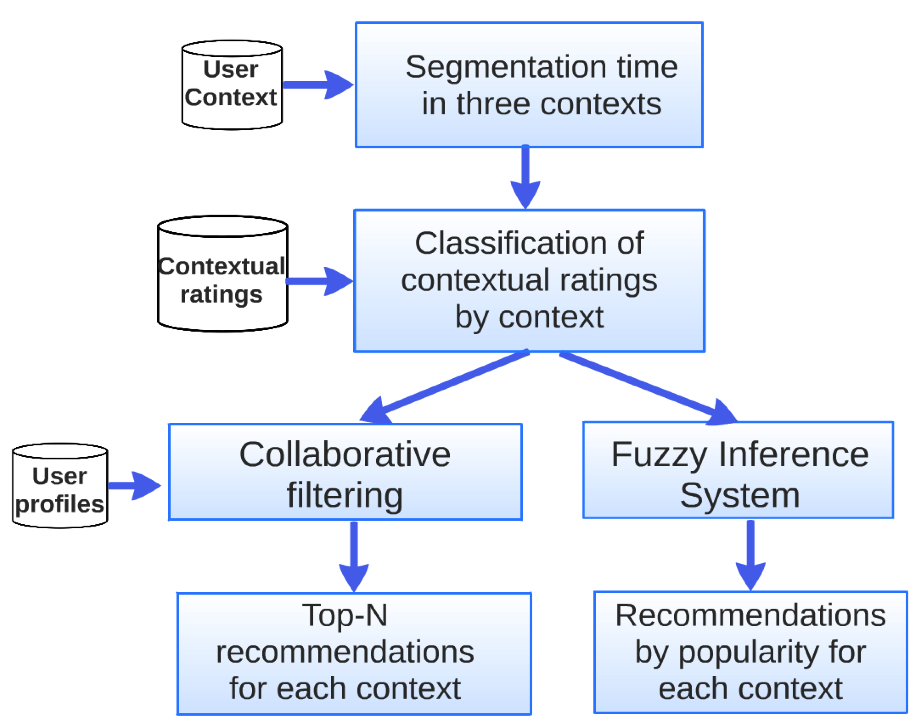
\includegraphics[width=0.50\textwidth]{img/archi-ml.png}
\caption{Pre-filtering approach used for Movielens dataset.}
\label{fig:archi-ml}     
\end{figure*}
The dataset used to test the algorithm was MovieLens(100000 ratings)
with 943 users and 1,682 movies. The ratings were collected in a
period  of 2 years. \\MovieLens is not a contextual dataset, however,
the  timestamp was used to determine the rating time, i.e., in this
way it  was noted the day to know whether the rating time was in
weekday or  weekend. In this terms, the context was used. Then, the
time for each  context was divided in 3 months each one, this span
covers 9 months  before the user's current context. \\ The neighbors
in each context are  considered to recommend movies in that context
only.  An average of  predictions are considered for add a movie to
the top-N list of contextualized recommendations. \\ The result in
table \ref{tab:contexts} shows the error in three contexts. The
error increase in context 3, in this  context the ratings matrix is a
little bit sparse;  the error is  justifiable because user has less
participations.
\begin{table}
\small
\captionsetup{font=footnotesize}
\caption{Results of comparison by contexts in MovieLens dataset.}
\label{tab:contexts} 
\small
\centering
\begin{tabular}{llll}
\hline\noalign{\smallskip}
Context & \# Preditions & MAE &    \\
\noalign{\smallskip}\hline\noalign{\smallskip}
1 & 12235 & 0.28 \\
2 & 21049 & 0.24 \\
3 & 1075  & 0.38 \\
\noalign{\smallskip}\hline
\end{tabular}
\end{table}
GroupLens Research has collected and made available rating data sets
from the MovieLens Web site (\url{http://movielens.org}). 

\subsection{TripAdvisor collection} 

The proposed method consists of three algorithms to recommend: 
\textit{fuzzy inference system}, \textit{collaborative filtering} and 
\textit{content-based}. Each one
uses the ratings matrix to get recommendations.\\    
The context-aware recommender system uses the \textit{post-filtering}
paradigm\cite{adomavicius2011context} for adjust recommendations in
context. The recommendation by popularity is through the fuzzy
inference system depicted in figure \ref{fig:fis}, the fuzzy inference
system contains the variables that are involved in the process to
recommend in a human interaction, this process is the same that the
recommender system does. \\The output represents how matter each item
into the users community, i.e. if it is a popular item between users. \\
The dataset used to evaluate the algorithm was TripAdvisor in two
versions downloaded\cite{linkzeng}, this datasets was used in
\cite{zheng2014context} and \cite{zheng2012differential} to  evaluate the
performance of context-aware recommender systems. \\The first
dataset contains 4669 contextual ratings, 1202 users and 1890 hotels;
the second dataset contains 14175 contextual ratings, 2731 users and
2269 hotels. Data were collected of reviews online in tripadvisor.com.
There is only one context: \textit{type of trip} (family, friends, bussines,
romantic and relax).\\ 
The FIS has Gaussians membership functions and are depicted in figure
\ref{fig:mffis}.
\begin{figure}[ht!]
   \captionsetup{font=footnotesize}
   \centering
   %%----primera subfigura----
   \subfloat[]{
        \label{fig:1a}
        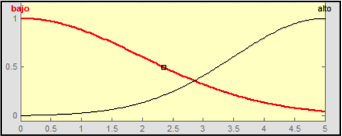
\includegraphics[width=0.42\textwidth]{img/ratingaverage.png}}
   \hspace{0.1\linewidth}
   %%----segunda subfigura----
   \subfloat[]{
        \label{fig:1b} 
        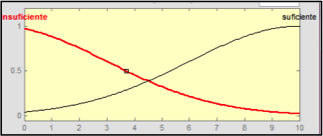
\includegraphics[width=0.42\textwidth]{img/userparticipation.png}}\\[20pt]
   %%----tercera subfigura----
    \subfloat[]{
        \label{fig:1c} 
        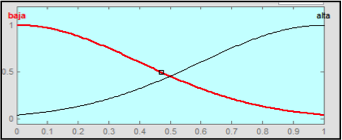
\includegraphics[width=0.42\textwidth]{img/recommendation.png}}
   \caption{Gaussian Membership functions in the input are: a) RatingAverage, 
   b) UserParticipation, and an output: c) Recommendation.}
   \label{fig:mffis} 
\end{figure}
The fuzzy inference system uses fuzzy rules to infer the inputs and 
output(a crisp value) that represents the weight of the recommendation. 
The rules are following: 
\begin{enumerate}
\item \textit{If \textbf{RatingAverage} is low and 
\textbf{UserParticipation} is insufficient then \textbf{recommendation} is low.}
\item \textit{If \textbf{RatingAverage} is low and 
\textbf{UserParticipation} is sufficient then \textbf{recommendation} is high.}
\item \textit{If \textbf{RatingAverage} is high and 
\textbf{UserParticipation} is insufficient then \textbf{recommendation} is low.}
\item \textit{If \textbf{RatingAverage} is high and 
\textbf{UserParticipation} is sufficient then \textbf{recommendation} is high.}
\end{enumerate}
\begin{figure*}
\captionsetup{justification=centering,margin=2cm,font=footnotesize}
\centering
\setlength\fboxsep{0pt}
\setlength\fboxrule{0.7pt}
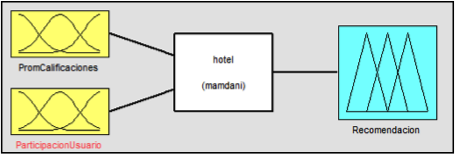
\includegraphics[width=0.75\textwidth]{img/fis.png}
\caption{Fuzzy Inference System.}
\label{fig:fis}   
\end{figure*}
Content-based uses cosine similarity to compare the binary
vectors representing the profile of each item, thereby obtaining a
numerical value that determines similarity, based on a threshold. \\   In
other words, it makes a comparison of profiles of each item to
determine the most similar to items the user has rated with highest
score, context-aware recommender system proposed has a scale from 1 to
5. 
\begin{table}[htb]
\small
\centering
\captionsetup{font=footnotesize}
\caption{Example of contextual ratings in the user profile.}
\label{tab:2}
\small
\begin{tabular}{lll}
\hline
\multicolumn{3}{c}{\textbf{User profile}} \\ \hline
Item & Rating & Context \\ \hline
La Casa del Mole & 5.0 & Midweek \\ 
Daruma           & 4.0 & Weekend \\ 
Daruma           & 5.0 & Midweek \\ 
Carl's Jr.       & 3.0 & Weekend \\ \hline
\end{tabular}
\end{table}
In the next step the outputs of every recommender algorithm is
represented by a list of recommended items. Subsequently applies the
context filter and context-aware recommender system gets the final
contextual recommendations. Context-aware
recommender system identifies contextual data of the user profile (see
table \ref{tab:2}), and compares recommended items to filter those
items that are adjusted to the user context. 
The context filtering is the last step before to get the recommended
items. The schema of architecture for context-aware recommender system
is depicted in figure \ref{fig:architecture}.
\begin{figure*}
\captionsetup{font=footnotesize}
%\captionsetup{justification=centering,margin=2cm}
\centering
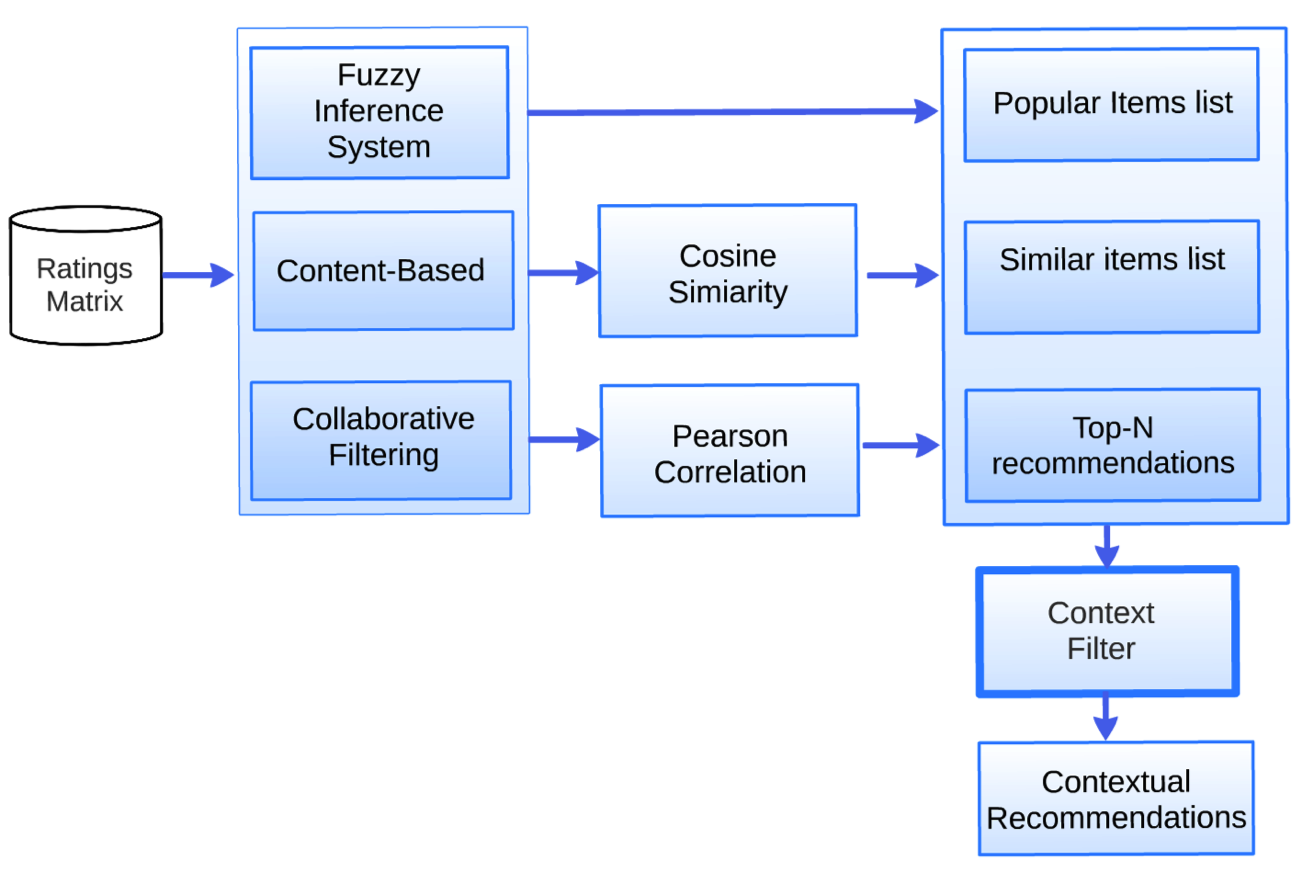
\includegraphics[width=0.80\textwidth]{img/archit-ta.png}
\caption{Recommender system methodology.}
\label{fig:architecture}   
\end{figure*}
Two experiments were performed using TripAdvisor dataset, table
\ref{tab:3} describes the data sets and the scarcity percentage of the
specified data. Scarcity of 99\% mean that there are problems to
recommend items because the information is not enought to get 
good recommendations.\\  By other side, in table \ref{tab:4} the comparison
shows that the algorithm has a acceptable performance, i.e., the error
falls into the range of results obtained with others algorithms. Then,
contextual recommendations were evaluated with the Root Mean Square
Error in order to compare the results with context relaxation
algorithm\cite{zheng2012differential} that is evaluated with the same
dataset.
\begin{table}
\centering
\small
\captionsetup{font=footnotesize}
\caption{Datasets description.}
\label{tab:3}      
\begin{tabular}{lllll}
\hline\noalign{\smallskip}
Dataset & Users & Items & Ratings & Scarcity (percent) \\
\noalign{\smallskip}\hline\noalign{\smallskip}
TripAdvisor v1 & 1202 & 1890 & 4669 & 99.79 \\
TripAdvisor v2 & 2731 & 2269 & 14175 & 99.77 \\
\noalign{\smallskip}\hline
\end{tabular}
\end{table}

\begin{table}
\centering
\small
\captionsetup{font=footnotesize}
\caption{Comparison of RMSE.}
\label{tab:4}  
\small   
\begin{tabular}{lll}
\hline\noalign{\smallskip}
Dataset & Algorithm & RMSE \\
\noalign{\smallskip}\hline\noalign{\smallskip}
TripAdvisor v2 & FC + Post-filtering  & 0.504  \\
               & FC          & 0.994  \\
               & Pre-filtering + Relaxation & 0.985  \\
\noalign{\smallskip}\hline
\end{tabular}
\end{table}
The cosine similarity plays an important role in content-based because
if similarity value among items is high, the recommendations will
improve the degree of user satisfaction. \\ This is observed when
calculating the similarity average in each dataset as shown in table
\ref{tab:5}.
\begin{table}
\centering
\small
\captionsetup{font=footnotesize}
\caption{Level of similarity among items in datasets. }
\label{tab:5}      
\begin{tabular}{lll}
\hline\noalign{\smallskip}
Dataset  & Similarity  & Avg.votes per user. \\
\noalign{\smallskip}\hline\noalign{\smallskip}
TripAdvisor v1 & 0.448  & 5  \\
TripAdvisor v2 & 0.508  & 8  \\
\noalign{\smallskip}\hline
\end{tabular}
\end{table}
FIS can provides a list of popular items for each dataset,
recommendations through averages are obtained, and recommendations are
conditioned to show it when the collaborative filtering and content-
based are not delivering recommendations because of data scarcity.\\ 
However, the majority of popular items of dataset were rated in contexts: romantic, family and bussines, that means that the dataset has
biases.\\  In this experiment  the context-aware recommender system
proposed involves the paradigm of post-filtering for contextual
recommendations. The structure of the datasets facilitated the
evaluation of recommendations although the rating matrix has been
scarce in both cases. Anyway, information of items and users was used
to test the system and a good performance of the system was done.\\   
With respect the performance, post-filtering allows select relevant
items that are adjusted into the context, indeed, post-filtering and
implementation of different recommendation techniques the system has
suitable performance and the datasets help the processes performed.

\subsection{Filmtrust and InCarMusic} 
%cambiar al nombre representativo del paper.
FilmTrust is a small dataset crawled from the entire FilmTrust website
in June, 2011. Filmtrust contains a ratings matrix of 35498 ratings,
1504  users and 2071 movies. \\ The dataset has a density of 1.14\% and
was used in \cite{guo2013novel} using the trust level such as
context. The web page is \url{http://www.librec.net/datasets.html}.\\ 
InCarMusic dataset\cite{baltrunas2011incarmusic} has 8 
contextual factors and the possible values for contextual conditions 
are explained in table \ref{tab:incarmusic}.\\ 
\begin{table}
\centering
\small
\captionsetup{font=footnotesize}
\caption{Contexts in InCarMusic dataset.}
\label{tab:incarmusic}   
\begin{tabular}{ll}
\hline\noalign{\smallskip}
Context  			& Values \\
\noalign{\smallskip}\hline\noalign{\smallskip}
Driving style 		&  elaxed, driving, sport driving.   \\
Road type 			&  city, highway, serpentine. \\
Landscape 			& coast line, country side, mountains/hills, urban.\\
Sleepiness 			& awake, sleepy. \\
Traffic conditions 	& free road, many cars, traffic jam. \\
Mood 				& active, happy, lazy, sad. \\
Weather 			& cloudy, snowing, sunny, rainy. \\
Natural phenomena 	& day time, morning, night, afternoon. \\
\noalign{\smallskip}\hline
\end{tabular}
\end{table}
Music tracks were ten different genres. There is not unified music
genre taxonomy, for this reason the recommender system uses the genres
defined in \cite{tzanetakis2002musical}: classical, country, disco, 
hip hop, jazz, rock, blues, reggae, pop and metal, 50 music tracks 
and 42 users in dataset.

\subsubsection{Results} 

For experiments with matrix factorization technique the \textit{Graphlab
toolbox} was used. FilmTrust, InCarMusic and Movielens (1 millon and
10 millions) were used to test the algoritmh. The test involves \textit{K
factors} that are increasing for \textit{50 iterations}.\\ Previously, was 
done a test to identify what number of iterations are enough to get a good
result with no overload of process in the algorithm. \\ Results are
depicted in the chart \ref{fig:fm-test} where the \textit{axis (x, y)}
represent the \textit{K value} and the \textit{error value}, respectively. 
The observations deal to small differences among the datasets, in a range
of \textit{0.80-0.90}, and the high variability is in \textit{MovieLens} 10
millions. Thus, the large dataset implies more unstable 
behaviour, while in a small dataset(Filmtrust) the error is less variable.
A comparison among MovieLens 1 million and 10 millions shows that 
there's not a significant difference. \\ 
By other side, another datasets were used to test matrix factorization
under the same parameters to calculate the RMSE for each one.\\ Table
\ref{tab:mf-set} presents the total of ratings of each dataset, the
cosine similarity that means how similar are the items into the
dataset, and the RMSE error obtained in the test with matrix
factorization technique, the datasets contain less number of ratings than
the presented in the chart \ref{fig:fm-test}. 
\begin{table}
\centering
\small
\captionsetup{font=footnotesize}
\caption{RMSE of datasets using matrix factorization.}
\label{tab:mf-set}   
\begin{tabular}{llll}
\hline\noalign{\smallskip}
Dataset & Ratings & Cosine Sim. & RMSE \\
\noalign{\smallskip}\hline\noalign{\smallskip}
Tijuana Rest.  &    896       &  0.67    &   0.60 \\
Mexico Rest.  &   1161       &  0.25    &  0.54 \\
InCarMusic    &    4012      &  0.45     &  0.93 \\
TripAdvisor    &    4669      &  0.17     &  0.85 \\
MovieLens    &    10000     &   0.46    &  0.51 \\
Movielens    &     100000   &   0.94    &  0.42 \\
\noalign{\smallskip}\hline
\end{tabular}
\end{table}
\begin{figure*}
\captionsetup{font=footnotesize}
\centering
\fbox{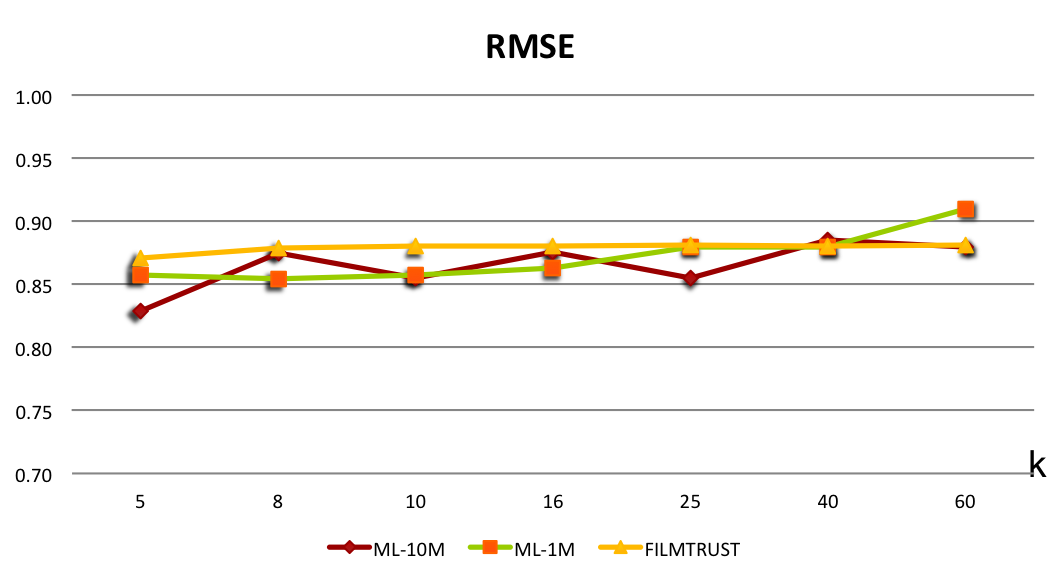
\includegraphics[width=0.70\textwidth]{img/fm-test.png}}
\caption{RMSE results of matrix factorization.}
\label{fig:fm-test}   
\end{figure*}
Making a comparison 
and according the table \ref{tab:mf-set} is not possible 
to affirm that matrix factorization has a better performance 
with small datasets, because TripAdvisor and InCarMusic datasets 
obtain a similar error in the same range that the large datasets.



